\chapter{Costs, Expected Utility and Deterrence}
\label{ch:becker}

\section{Becker's question}

In 1968 Gary Becker published \emph{Crime and Punishment: An Economic Approach}, which treated criminal behaviour as a choice made in response to expected costs and benefits, and the design of criminal law as a problem of minimising social loss \citep{becker1968}. The idea began, by Becker's own account in his Nobel lecture \citep{becker1993}, with a decision about whether to park illegally on the way to an oral examination: he weighed the probability of a ticket and its cost against the inconvenience of finding a legal space, and parked illegally. If he reasoned that way, he thought, perhaps criminals did too, and perhaps the law should be designed with that in mind.\index{Becker, Gary}\index{deterrence}

Becker's approach, extended with Kevin Murphy and others at Chicago, is expected utility theory applied to the law. The potential offender maximises expected utility, choosing whether to offend given the probability of conviction and the severity of punishment. The state chooses the probability and severity, through spending on police and courts and through the sentencing law, to minimise the sum of the harm from crime and the costs of enforcement and punishment. This chapter sets out Becker's model and its main implications, the extension by Becker, Murphy and Grossman to markets for illegal goods, and the economics of litigation and settlement, which is where the costs of the courts themselves enter.

\section{The model}

\subsection{The offender}

A potential offender gains $g$ from an offence. If caught and convicted, which happens with probability $p$, he suffers a sanction $f$, measured in money or its equivalent. With utility function $u$ over wealth $w$, he offends if
\begin{equation}
p\,u(w + g - f) + (1-p)\,u(w+g) > u(w).
\end{equation}
For a risk neutral offender this reduces to $g > pf$: he offends when the gain exceeds the expected sanction. The supply of offences in a population is the number of people for whom this inequality holds, $O(p, f)$, decreasing in both $p$ and $f$.

\subsection{Social loss}

The state chooses $p$ and $f$ to minimise
\begin{equation}
L(p,f) = D(O) + C(p, O) + b\,p\,f\,O,
\label{eq:beckerloss}
\end{equation}
where $D(O)$ is the net harm from $O$ offences, $C(p,O)$ the cost of apprehending and convicting with probability $p$, and $b\,p\,f\,O$ the social cost of punishment, with $b$ measuring how costly a unit of sanction is to society. For a fine, $b$ is near zero, since a fine is a transfer; for imprisonment, $b$ is large, since prison is costly to run and destroys the prisoner's productivity.\index{social loss}

\subsection{Implications}

Several implications follow.

\paragraph{High sanctions, low probabilities} Raising $p$ is costly, since it requires more police and courts. Raising $f$ is cheap when the sanction is a fine. A risk neutral offender responds to $pf$, so the same deterrence can be achieved with a lower $p$ and a higher $f$ at lower cost. Becker concluded that, for fines, the optimal policy sets $f$ as high as the offender's wealth permits and $p$ correspondingly low. Figure~\ref{fig:becker} shows curves of constant expected sanction in the $(p,f)$ plane; the cheapest point on each curve has low $p$.

\begin{figure}[t]
\centering
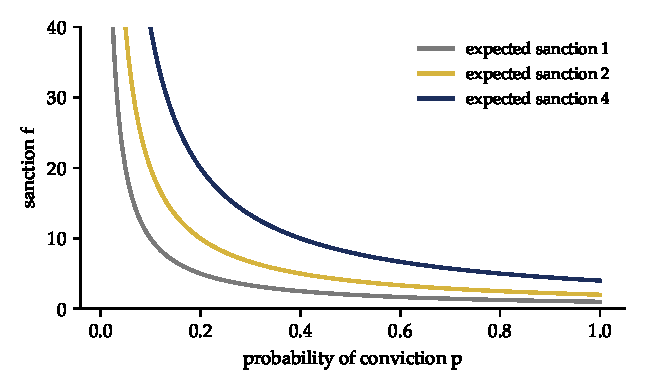
\includegraphics[width=\linewidth]{fig_becker}
\caption{Combinations of the probability of conviction and the sanction that give the same expected sanction. If raising the probability is costly and the sanction is cheap, the efficient point on each curve lies to the left.}
\label{fig:becker}
\end{figure}

\paragraph{Limits} The conclusion is limited by wealth, since fines cannot exceed what the offender can pay; by attitudes to risk, since a risk averse offender is deterred more by severity than by certainty but bears a real cost from an uncertain sanction, while a risk preferring offender is deterred more by certainty than by severity; by the cost of imprisonment when fines are infeasible; and by marginal deterrence, the point, developed by Stigler, that if minor crimes are punished as severely as major ones, offenders have no incentive to stop at the minor crime \citep{stigler1970}. It is also limited by error. Chapter~\ref{ch:standards} showed that the losses from false convictions shape the standard of proof. When sanctions are severe, the loss from a false conviction rises, so the threshold for conviction should rise, which lowers $p$ further for the guilty. Severe sanctions and a high standard of proof interact.\index{marginal deterrence}

\paragraph{Error and deterrence} Errors reduce deterrence. If the probability of conviction for the guilty is $p_G$ and for the innocent is $p_I$, then the difference in expected sanction between offending and not offending is $(p_G - p_I)f$ \citep{kaplow1994}. False convictions of the innocent reduce the deterrent effect of punishment, because they impose sanctions whether or not one offends. Accurate fact finding therefore has deterrent value beyond its fairness value. A more accurate court that reduces $p_I$ while holding $p_G$ fixed increases deterrence at no cost in sanctions.

\section{Enforcers' incentives}

Becker and Stigler extended the analysis to the incentives of those who enforce the law \citep{becker1974}. Police, prosecutors and regulators can be bribed, and an enforcer who takes bribes undermines deterrence. They proposed paying enforcers above market wages, with a bond forfeited on discovery of malfeasance, so that honest service is worth more than a bribe. The analysis applies to the expert witnesses and court officials of earlier chapters: their reports are signals, and their incentives determine the signals' reliability. The selection of favourable experts discussed in Chapter~\ref{ch:fienberg} is a version of the enforcer problem.

\section{The market for illegal goods}

\subsection{Becker, Murphy and Grossman}

In 2006 Becker, Murphy and Grossman analysed the market for illegal goods, using drugs as their example \citep{bmg2006}. Enforcement against suppliers raises their costs: they must evade detection, pay for violence and accept the risk of punishment. Higher costs raise prices and reduce consumption. The question is how much enforcement is optimal, and the answer depends on the elasticity of demand.

Suppose enforcement raises the price of the illegal good. If demand is elastic, with absolute elasticity greater than one, consumption falls proportionately more than price rises, and total spending on the good falls. If demand is inelastic, consumption falls proportionately less, and total spending rises. Since much of the cost of an illegal market is the resources suppliers spend on evasion and violence, and these scale with revenue, enforcement against an inelastically demanded good can increase the social costs of the market while reducing consumption only modestly. Figure~\ref{fig:bmg} shows the sign change at unit elasticity.\index{illegal goods}\index{drugs, market for}

\begin{figure}[t]
\centering
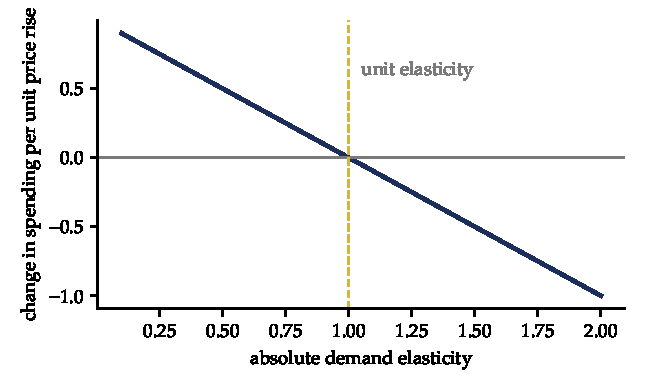
\includegraphics[width=\linewidth]{fig_bmg}
\caption{The change in total spending on an illegal good per unit increase in its price, relative to quantity, as a function of the absolute elasticity of demand. Below unit elasticity, enforcement that raises the price raises total spending.}
\label{fig:bmg}
\end{figure}

Becker, Murphy and Grossman showed that optimal enforcement is lower when demand is less elastic, and that, for goods with inelastic demand, a legal market with a tax could reduce consumption more cheaply than prohibition, because a tax raises the price without inducing the costly evasion and violence that enforcement does. Their analysis did not depend on any particular view of the morality of drug use; it took the reduction of consumption as the goal and asked how to achieve it at least cost.

\subsection{Rational addiction}

Becker and Murphy's earlier theory of rational addiction modelled addictive consumption as a choice by forward looking individuals whose current consumption raises the marginal utility of future consumption \citep{becker1988}. Addicts in the model respond to expected future prices, so permanent price increases reduce consumption more than temporary ones, and announced future enforcement affects current behaviour. Whether addicts are as forward looking as the model assumes is debated, but the empirical evidence that cigarette consumption responds to expected future prices supports at least part of the theory \citep{becker1994}. For legal policy the implication is that the credibility and persistence of enforcement matter: a temporary crackdown has less effect than a durable change.

\subsection{Social interactions}

Becker and Murphy's \emph{Social Economics} studied how individuals' choices depend on those of others through norms, peer effects and social multipliers \citep{becker2000}. Crime is a leading example. Glaeser, Sacerdote and Scheinkman showed that the variance of crime rates across American cities is far larger than individual characteristics can explain, and attributed the excess to social interactions in which one person's offending raises the probability that others offend \citep{glaeser1996}. With social multipliers, a policy that deters some offenders has indirect effects on others, and the total effect of enforcement exceeds its direct effect. Estimation of social multipliers is difficult, because peers' choices are correlated for many reasons, but it is necessary for any honest estimate of the effect of enforcement.

\section{Valuing life and harm}

Damages in tort and the harm from crime must be measured. For injuries to life and health, economists use the value of a statistical life, inferred from the wages workers accept for risky jobs and the prices people pay for safety. Murphy and Topel estimated the social value of improvements in health and longevity in the United States and found them enormous: longevity gains from 1970 to 2000 were worth about 3.2 trillion dollars a year, and the gains of the twentieth century over 1.2 million dollars per person \citep{murphy2006}. The value of a statistical life used by American regulatory agencies is of the order of ten to fourteen million dollars: the Department of Transportation's current figure is about \$14.2 million (base year 2025) \citep{dot2025}. Courts generally do not use these figures directly, but the method, which infers a valuation from choices under risk, is the expected utility approach applied to the measurement of loss.

\section{Punitive damages and the multiplier}

If a defendant who causes harm $H$ is held liable with probability $q < 1$, then compensatory damages of $H$ impose an expected cost of $qH$, less than the harm. The defendant underinvests in care. Polinsky and Shavell argued that punitive damages should make up the difference, so that total damages equal $H/q$: if only one in four injured parties sues and wins, damages should be four times the harm \citep{polinsky1998}. This is Becker's logic applied to tort. It implies that punitive damages should depend on the probability of escaping liability, not on the reprehensibility of the conduct as such, which is the factor American courts emphasise. The Supreme Court in \emph{State Farm v Campbell} suggested that few awards exceeding a single digit ratio between punitive and compensatory damages would satisfy due process \citep{statefarm2003}. In the Polinsky and Shavell framework, a ratio of nine to one corresponds to a probability of liability of one in ten.\index{punitive damages}

\section{The economics of litigation}

\subsection{Why cases settle}

Most civil disputes settle. A trial costs both parties money and time, and if they agreed on the probable outcome they could split the savings. The basic model, due to Landes, Gould (the economist John P. Gould, not the sociologist Roger Gould) and Posner \citep{landes1971,gould1973,posner1973}, says that a case goes to trial only if the parties' expectations diverge enough to overcome the costs. Let the claimant (the plaintiff, in the language of the next subsection) believe it will win with probability $p_P$ and the defendant believe the claimant will win with probability $p_D$. The judgment if the claimant wins is $J$, and the parties' trial costs are $C_P$ and $C_D$. The claimant will accept any settlement above $p_P J - C_P$, and the defendant will pay up to $p_D J + C_D$. Settlement is possible if
\begin{equation}
p_P J - C_P \le p_D J + C_D, \quad\text{that is}\quad (p_P - p_D)\,J \le C_P + C_D .
\label{eq:settle}
\end{equation}
Trials occur when the parties' optimism, $p_P - p_D$, multiplied by the stakes, exceeds the combined costs. Figure~\ref{fig:settlement} shows the settlement zone shrinking as the gap between beliefs grows.\index{settlement}

\begin{figure}[t]
\centering
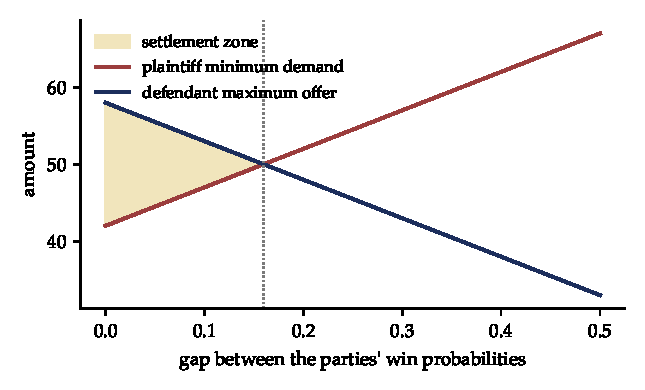
\includegraphics[width=\linewidth]{fig_settlement}
\caption{The claimant's minimum acceptable settlement and the defendant's maximum offer, as functions of the gap between their estimates of the claimant's chance of winning, with stakes of one hundred and costs of eight each. A settlement zone exists only to the left of the dotted line.}
\label{fig:settlement}
\end{figure}

\subsection{Priest and Klein}

Priest and Klein drew a striking implication \citep{priest_klein1984}. If both parties form estimates of the outcome with noise, and cases go to trial only when the estimates diverge, then the cases that are tried are disproportionately those close to the decision standard, where small errors in estimation lead to large disagreements. Cases far from the standard, which one side will clearly win, settle. Among tried cases, plaintiffs should therefore win about half the time, regardless of the underlying distribution of case quality, when the stakes are symmetric. Figure~\ref{fig:priestklein} shows a simulation in which plaintiff win rates at trial approach one half as the noise in the parties' forecasts falls.\index{Priest and Klein}\index{selection of disputes}

\begin{figure}[t]
\centering
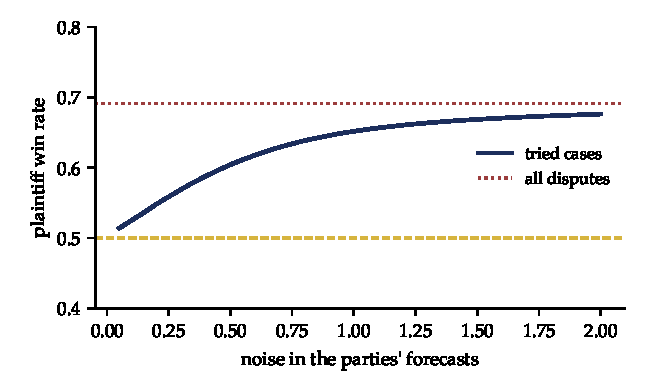
\includegraphics[width=\linewidth]{fig_priest_klein}
\caption{Plaintiff win rate among tried cases as a function of the noise in the parties' forecasts, in a simulation of the Priest and Klein model. Case quality is normal with mean $0.5$ and unit variance, the plaintiff wins if quality is positive, and a case is tried when the parties' estimated win probabilities differ by more than $0.3$, the ratio of combined costs to stakes. Plaintiffs win $69$ per cent of all disputes (dotted line), but the win rate at trial falls toward one half as forecasts become accurate.}
\label{fig:priestklein}
\end{figure}

The Priest and Klein hypothesis has an important implication for any attempt to learn the law from decided cases, including the machine learning approaches of Chapter~\ref{ch:pleadings}. Decided cases are a selected sample of disputes, enriched for close cases. A model trained on them will overestimate how uncertain the law is and will misjudge the outcomes of cases that typically settle. A Bayesian model that represents the selection process explicitly can correct for this; one that ignores it cannot.

\subsection{Asymmetric information}

Bebchuk modelled settlement when one party has private information about the case, in his model the defendant knows the plaintiff's chance of winning and the uninformed plaintiff makes a take-it-or-leave-it demand \citep{bebchuk1984}. The uninformed party makes an offer that some informed types accept and others reject, and trials occur because of the screening, not only because of optimism. In this model trials are a cost of asymmetric information. Discovery reduces asymmetry and so promotes settlement, which is one rationale for broad discovery rules, offset by their cost, as \emph{Twombly} emphasised \citep{twombly2007}.

\subsection{Who pays the costs}

Under the American rule each party bears its own legal costs; under the English rule the loser pays the winner's reasonable costs. The English rule raises the stakes of trial for both sides and makes the outcome matter more. In the optimism model it makes settlement less likely for parties who are both optimistic, because each expects the other to pay its costs, and it deters weak claims, since a claimant with a low probability of success faces paying the defendant's costs. Empirical comparisons are difficult, but the analysis \citep{shavell1982} shows that cost rules are instruments that change the distribution of disputes that reach trial.

\section{Plea bargaining}

In the United States the great majority of criminal convictions result from guilty pleas, typically in exchange for reduced charges or sentences. In a Becker style model, the defendant accepts a plea if the certain sentence $s_{\text{plea}}$ is less than the expected sentence at trial, $\Prob(\text{convict})\,s_{\text{trial}}$, adjusted for risk aversion. The prosecutor offers a plea to economise on trial costs. The problem is that an innocent defendant with a modest probability of conviction may rationally plead guilty if the trial sentence is severe enough. If the probability of wrongful conviction at trial is twenty per cent and the trial sentence is ten years, an innocent defendant who is risk neutral would accept a plea to any sentence below two years.\index{plea bargaining}

A Bayesian view of plea bargaining emphasises that the plea offer reveals information. A prosecutor who offers a large discount signals that her case is weak, and a defendant who rejects a generous offer signals confidence in his innocence or his defence. Grossman and Katz analysed plea bargaining as a screening device that sorts defendants by guilt \citep{grossman1983}. Whether the sorting is good depends on the size of the trial penalty. When the penalty for going to trial is large, the screening breaks down, because innocent and guilty defendants alike plead. Reforms that limit the gap between plea and trial sentences protect the innocent at the cost of more trials.

\section{The cost of the courts}

The Becker framework treats courts as a cost of producing $p$, the probability of conviction. Much of this book has been concerned with reducing that cost or improving the accuracy of what it buys. Chapter~\ref{ch:india} showed what happens when the cost is not met: delay becomes a tax on all litigants and a punishment of the accused. The Bayesian contribution to Becker's program is to model the production of $p$ explicitly, as the result of evidence gathering and inference, so that improvements in inference, such as better forensic statistics, explicit likelihood ratios and machine triage, can be valued in the same units as more police or harsher sentences. A reform that raises the accuracy of verdicts raises deterrence and reduces the harm of false convictions at the same time. That is a strong economic argument for Bayesian courts.

\section*{Notes and Questions}
\addcontentsline{toc}{section}{Notes and Questions}
\begin{enumerate}[label=\arabic*.]
\item In Becker's model with risk neutral offenders, suppose $D(O) = O$, $C(p) = c\,p^2$ with $c = 4$, $O$ is the fraction of the population that offends, fines are costless ($b = 0$) and offenders' gains are uniform on $[0, 10]$. If the maximum fine is $20$, what $p$ minimises social loss?
\item Show that if offenders are risk averse, increasing $f$ while holding $pf$ constant increases deterrence. What does this imply for the optimal mix of $p$ and $f$?
\item In the Becker, Murphy and Grossman analysis, explain why enforcement against a good with inelastic demand can increase the resources devoted to the illegal market.
\item Using \eqref{eq:settle}, with $J = 100$, $C_P = C_D = 10$, find the largest optimism gap at which settlement is possible. How does the English rule change the analysis if the loser pays both parties' costs?
\item A defendant believes there is a thirty per cent chance of conviction at trial, where the sentence would be eight years. What plea offers would a risk neutral defendant accept? How does your answer change if he is risk averse?
\item Explain the Priest and Klein hypothesis in your own words. What does it imply about using appellate decisions to estimate the probability that a type of claim will succeed?
\end{enumerate}

\section*{Further reading}
Becker's 1968 paper \citep{becker1968}; Becker, Murphy and Grossman on illegal goods \citep{bmg2006}; Polinsky and Shavell on public enforcement and on punitive damages \citep{polinsky2000,polinsky1998}; Priest and Klein on the selection of disputes \citep{priest_klein1984}.
